\documentclass[a4paper, titlepage]{article}

\usepackage[ngerman]{babel}
\usepackage[T1]{fontenc}
\usepackage[utf8]{inputenc}
\usepackage{graphicx}
\usepackage{amsmath}
\usepackage{tabularx}


\title{Die Gravitationskonstante g
auf einer schiefen Bahn}
\author{Sascha Huber, Aaron Stampa, Joanne Gautschi, Damien Flury}
\date{1. Dezember 2019}
\begin{document}
    \maketitle
    \tableofcontents
    \newpage
    \section{Experiment}
    Wir haben unser Experiment eingerichtet, wie auf Abbildung
    \ref{incline} dargestellt. Dann haben wir verschiedene Objekte
    herunterrollen lassen mit verschieden Höhen
    \emph{h}. Die Länge \emph{x} ist die Distanz, in welcher
    wir die Objekte messen. Der Winkel $\theta$ bezeichnet
    den Winkel der schiefen Ebene in Bogenmass.

    \subsection{Ball auf der schiefen Ebene}
    Zunächst haben wir einen Ball herunterrollen lassen.
    Sein Radius \emph{r} beträgt etwa 4 cm, seine Masse
    \emph{m} 242 g.
    
    Wir haben die Strecke \emph{s} in Abhängigkeit
    der Zeit \emph{t} gemessen, um die Beschleunigung
    \emph{a} zu bestimmen. Dazu haben wir folgende Formel
    angewandt:
    \begin{align}
        s &= \frac{1}{2} \cdot a \cdot t^2 \\
        a &= \frac{2 \cdot s}{t^2} &\text{(Termumformung)}
    \end{align}


    \begin{figure}
        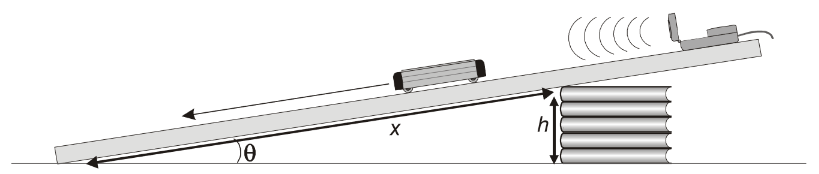
\includegraphics[width=\textwidth]{images/incline.png}
        \caption{Schiefe Bahn}
        \label{incline}
    \end{figure}

    \begin{table}
        \begin{tabularx}{\textwidth}{|X|X|X|X|X|X|X|}
            \hline
            \textbf{Number of books} & \textbf{Height of books $(m)$} & 
            \boldmath{$\sin{\theta}$} & \textbf{Trial 1 $(m/s^2)$} & 
            \textbf{Trial 2 $(m/s^2)$} & \textbf{Trial 3 $(m/s^2)$} & 
            \textbf{Average acceleration $(m/s^2)$} \\
            \hline
            3 & 0.115 & 0.0479 & 0.26 & 0.31 & 0.36 & 0.310 \\
            \hline
            4 & 0.144 & 0.0600 & 0.49 & 0.38 & 0.41 & 0.426 \\
            \hline
            5 & 0.174 & 0.726 & 0.60 & 0.45 & 0.38 & 0.476 \\
            \hline
            6 & 0.200 & 0.834 & 0.61 & 0.59 & 0.56 & 0.586 \\
            \hline
            7 & 0.275 & 0.115 & 0.97 & 1.22 & 1.22 & 1.137 \\
            \hline
        \end{tabularx}
    \end{table}


\end{document}